In this work, we apply a parameter fitting technique to validate a hybrid agent-based model with available \textit{in vitro} experimental data in order to explore the best-fit values for the unknown parameters given in Table \ref{parameters}. The three unknown parameters are termed the free parameters and together they define the vector $\bar{P}=<K,\mu _{V},\beta>$. We use an error-minimization search approach that explores the space of free parameters and returns the vector $\bar{P}$ that yields the simulation results best fitting the experimental data \cite{qanitabaker:Vargis2014Effect}. The fitting process is summarized as follows:


\begin{description}
\item[\textbf{Given:}] \textit{   Model free parameters, simulation outputs, and experimental \textit{in vitro} data.}
\item[\textbf{Find}:] \textit{Best-fit values for the free parameters (best $\bar{P}$)}
\item[\textbf{Such}] \leavevmode  \textit{The error between the simulation and experimental \textit{in vitro} data is minimized.}
\\[-20pt] \item[\textbf{That}:]

%\item[\textbf{Such That:}] \textit{The error between the simulation and experimental \textit{in vitro} data is minimized.}

%\item[Condition:] Minimize the error between simualtion outputs and experimental \textit{in vitro} data.
\end{description}



\begin{figure}[!t]
\centering
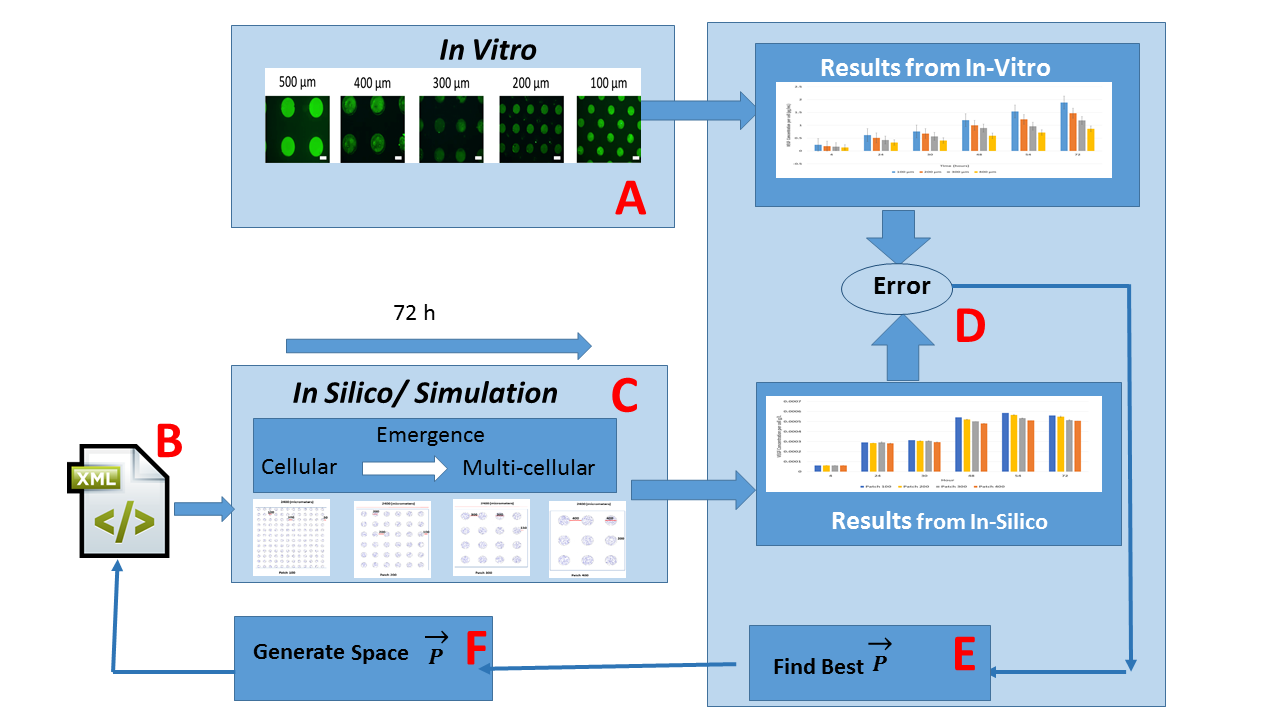
\includegraphics[width=3.5in]{./figures/Overview.png}

\caption{An overview for the error-minimization multicellular search-based approach. In (A), RPE cells are cultured using micropatterning techniques. In (B), the parameters are initialized in the XML protocol file. In (C), a simulation is performed and the results are calculated. In (D), the error is calculated based on the difference in VEGF concentration per cell between the experimental results and simulation outputs as in Equation \ref{Model error}. Based on the change in error, new parameter values are selected for another simulation run (E and F). This process(B-F) will be repeated until an exit condition is met where the error improvement is below a threshold value or the search time runs out.}
\label{Fittingoverview}
\end{figure}


The search for the correct $\bar{P}$ (described in Algorithm \ref{optimization_Algo} and Figure \ref{Fittingoverview}) starts by sweeping over an initial range of values for each free parameter being fitted. A single sweep consists of running simulations for the space of $\bar{P}$ (all combinations of free parameter values based on their ranges). The range is defined by a minimum value, a maximum value, and a step value. In a sweep, each parameter starts from its minimum value and incrementally increases to its maximum value by its step value. An error is calculated for each parameter vector  by comparing the time-series outputs of the simulation with experimental \textit{in vitro} data (see Figure \ref{Fittingoverview}D). The vector $\bar{P}$ of parameter values with the minimum error is selected and becomes the midpoint for the parameter ranges in the next sweep (see Figure \ref{Fittingoverview}E and F). The process continues until an exit condition is met where the reduction in error is below a threshold or the preset search time runs out. The parameter values (both free and known parameters) for a simulation are specified via the protocol file. (see Figure \ref{Fittingoverview}B).

In this model, the error was calculated using Equation \ref{Model error}. $V_{s}(i,t)$ and $V_{e}(i,t)$ are the VEGF concentrations per cell in the simulation and \textit{in vitro}, respectively; $i$ is the patch size, $i \in \{ 100, 200, 300, 400\mu m \}$ and $t$ is the time in hours, $t \in \{4, 24,30, 48, 54, 72$ hours $\}$. The model error ($\varepsilon m$) is the sum of the errors over the four patch sizes and six time points. The error was calculated for each parameter vector $\bar{P}$. Additionally, since the simulation process is stochastic, each simulation was repeated 10 times, starting from different random seeds, and the results averaged for all presented data. Here it is important to note that this approach could be used to fit other models using different parameters, experimental results, and error functions.



%The challenge is to determine the gradient function to map changes in the error functions (error) to changes in the model configuration (parameters). Hill-Climbing algorithm is used to perform this task by giving it the ability to choose the input parameters based on the changes in errors ($\Delta Error$).


\begin{equation}
 \varepsilon m = \sum_{i} \sum_{t}^{} (V_{e}(i,t)-V_{s}(i,t))^2\quad  \quad  | \bar{P}=<K,\mu _{V},\beta>
\label{Model error}
\end{equation}

%Where:
%\begin{itemize}
%    \item $\mu _{V}$: is the VEGF secretion rate of RPE cells.
%    \item $\beta$: is the VEGF coefficient (VEGF binding affinity).
%    \item $K$: is the auto regulation rate of VEGF.
%\end{itemize}


%An overview of the error-minimization search method is illustrated in Figure \ref{Fittingoverview}. For the experimental compartment model, an important objective is to minimize the error function between \textit{in vitro} data and simulated results. Computing this error function requires a computationally intensive process. This begins with running simulations using parameters generated through parameters’ sweep and the defined input XML protocol files (each file determines initial condition for the patches sizes arrangements). Next, the VEGF concentration per cells is calculated for each simulation through different time slots. Then, the error function is computed using VEGF concentration per cell based on several  runs as in Equation \ref{Model error}. Finally, the parameters' values are used to determine the nearby region to further refine solution quality. This process is repeated until an exit condition is met where the error improvement is below a defined threshold value or the search time runs out. Additionally, since the simulation process is stochastic, the error is averaged over 10 model executions for each XML protocol file, each starting from different random seeds. Higher fidelity models take into account the real domain size, and all parameters used in the protocol files are biologically realistic parameters, except the free parameters defined above.

\begin{algorithm}
\caption{Algorithm for the Error-Minimization Search-Based approach using parameter sweeps which identifies a parameters vector $\bar{P}$ that is locally optimal}
\label{optimization_Algo}
\begin{algorithmic}[1]

\State \textbf{Input}: List of Free-Parameters $P$, XML Protocol Files $P_{files}$, and realistic parameter ranges $Rs$.
\State For each parameter $p_k$ in $P$, initialize  $max_k$, $min_k$, $step_k$ randomly within $Rs$.
\While{\textit{time-out is not reached and $error_{change}$ $>$ $error_{threshold}$ }}
\State$SWEEP(P_{files}, 1, max_1, min_1, step_1, \{\}, 10)$ \Comment{Recursive parameter sweeping algorithm. Started with the first parameter. See Algorithm \ref{sweep_Algo}}
\State For each simulation result from the space of $\bar{P}$s, calculate the VEGF concentration per cell for each patch size $i$ and time $t$
\Comment {There are 10 repeats for each simulation using different random seeds}
\State Calculate the $average_{VEGF}$ concentration
\State Find the $error$ based on equation \ref{Model error}
\State $error_{change}$ = $error_{previous}$ - $error$
\If {$error$ $<$ $error_{lowest}$}
\State $error_{lowest}$ $=$ $error$
\Comment {Keep track of the lowest error found so far and the change in error from the last sweep}
\State Change $max_k$, $min_k$, $step_k$ based on parameter values associated with $error$
\EndIf
%\If {$error$ change is less than defined threshold}
%\State  For each parameter $P_i$ in $ \vec{p_in}^{} $, initialize  $p_imax$, $p_imin$, $p_istep$ randomly within $Rs$. \label{line}
% \EndIf
\EndWhile
\State Return the parameters values $\bar{P}$ associated with $error_{lowest}$  \Comment {this will return the best value(s) found}

\end{algorithmic}
\end{algorithm}



%In the \textit{in silico} model, $ \vec{p}^{} $ is a vector of three parameters with default initial random values defined within biological acceptance ranges. For each free parameter, start sweeping value, end sweeping value, and step are randomly selected from the parameters' legal ranges. The parameter sweep process determines the best parameter values that yield the local minimum error value, which is used to define the next sweep region (this step represent the refinement operator). If the error is larger than the threshold and the run does not exceed the time out, random values are generated by adding random noise. The main idea behind this approach is applying repetition parameters' sweeps based on the values gained from the previous sweeps. If the error does not change at some point then each value is randomly set from the parameters' legal range (restart random) as in line 2 in Algorithm \ref{optimization_Algo}.


\begin{algorithm}
\caption{The parameter sweep algorithm that performs a simulation for all $\bar{P}$ (a combination of free parameters). $P_{files}$ are the XML protocol files that define the model input and initial condition, $K$ is the parameter count, $k$ is a counter that ranges from 1 to $K$, $max_k$ is the maximum value for parameter $k$, $min_k$ is the minimum value for the $k$th parameter, and $step_k$ is the value by which parameter $k$ is incremented, $\bar{P}$ holds a single combination of parameter values for which a simulation will be performed, $P$ is a matrix of size $K$x$j$ where $j$ is the number of values in the range of some parameter (which changes as the algorithm progresses) and P[k][j] holds the jth value of the kth parameter, and $Run_N$ is the number of repeated runs, each using different random seeds }
\label{sweep_Algo}
\begin{algorithmic}[2]

\Procedure{Sweep}{$P_{files}$, $k$, $max_k$, $min_k$, $step_k$, $\bar{P}$, $Run_N$}


\If {$k = K$}
\State Generate XML Protocol Files $G_{Pfiles}$ with the same setup as in $P_{files}$ with the parameter values $\bar{P}$
    \State $Run (G_Pfiles,P_Set,Run_N)$   \Comment {random seeds runs}
%    \State $Run (G_Pfiles)$
    \State $\bar{P}.Empty$
\Else
    \State $j = 1$
    \State $P[k][j]=min_k-step_k$
    \While {$P[k][j]<max_k$}
       \State $P[k][j]=P[k][j]+step_k$
       \State $\bar{P}.Add(P[k][j])$
       \State $j = j + 1$
       \State $k = k + 1$
       \State $SWEEP(G_{Pfiles}, k, max_k,$
       \State $min_k, step_k,\bar{P}, 10)$
   \EndWhile
\EndIf





\EndProcedure

\end{algorithmic}
\end{algorithm}



